\documentclass[12pt]{standalone}
%\documentclass[crop,tikz,convert={outext=.svg,command=\unexpanded{pdf2svg \infile\space\outfile}},multi=false]{standalone}[29.03.2022]
\usepackage[left=2.5cm, right=4.5cm, top=2.5cm, bottom=2cm]{geometry}
\usepackage[onehalfspacing]{setspace}
\usepackage[utf8]{inputenc}
\usepackage{ngerman}
\usepackage{bibgerm}
\setlength\parindent{0pt}

\usepackage{graphicx}
\usepackage{subfig}
\usepackage{wrapfig}
\usepackage{caption}

\usepackage{sidecap}
\usepackage{tikz}
\usetikzlibrary{calc}
\usetikzlibrary{shapes,arrows}
\usetikzlibrary{arrows.meta}
\usepackage{environ}
\usepackage{tikz-3dplot}
\usepackage{import}
\usepackage{calc}
\usepackage{pgfmath}
\usepackage{ifthen}
\usepackage{pgfplots}
\usepgfplotslibrary{fillbetween}
\usepackage{amsmath}
\usepackage{makecell}
\usepackage{xr}
\usepackage{xurl}
\usepackage{footnote}
\usepackage[perpage, hang]{footmisc}
\usepackage{tablefootnote}
\usepackage{tabularx}
\usepackage{textcomp}
\usepackage[section]{placeins}
\usepackage{hyperref}
\setlength\footnotemargin{10pt}
\usepackage{listings}
\usepackage{chngcntr}
\usepackage{lipsum}
\usepackage{color, colortbl}
\usepackage{multirow}
\usepackage{float}
\usepackage[export]{adjustbox}
\newfloat{Ausschnitt}{htbp}{loa}
\newcommand{\captionref} [1]{\textit{\nameref{#1}}}
\newcolumntype{x}[1]{>{\centering\arraybackslash}p{#1}}
\usepackage{standalone}

\tikzset{%
  block/.style    = {draw, thick, rectangle, minimum height = 3em,
    minimum width = 3em},
  sum/.style      = {draw, circle, node distance = 1.5cm}, % Adder
  input/.style    = {coordinate}, % Input
  output/.style   = {coordinate}, % Output
   base/.style = {rectangle, rounded corners, draw=black, minimum width=2cm, minimum height=1cm, text centered}
}

\thispagestyle{empty}

\begin{document}

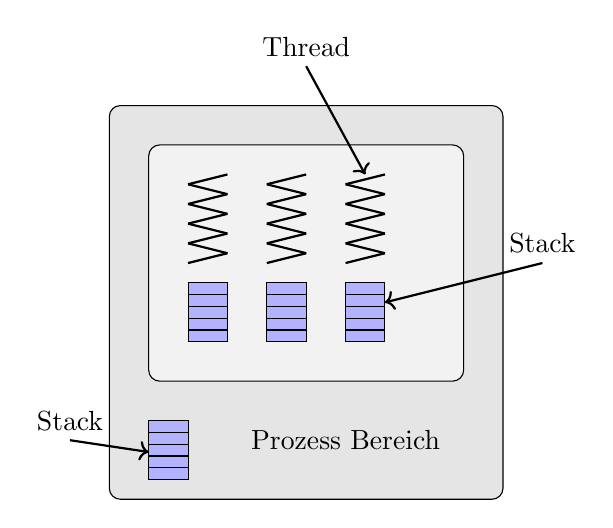
\begin{tikzpicture}[scale=0.5]
  \draw[rounded corners, fill=black!10] (0, 0) rectangle (10, 10){};
  \draw[rounded corners, fill=black!5] (9,9) rectangle (1, 3);

  \foreach \s in {0, 0.3, ..., 1.5}{
      \draw[fill=blue!30] (1, 0.5+\s) rectangle (2, 0.5+\s+0.3);
  }

  \foreach \s in {0, 0.3, ..., 1.5}{
      \draw[fill=blue!30] (2, 4+\s) rectangle (3, 4+\s+0.3);
  }
  \foreach \s in {0, 0.3, ..., 1.5}{
      \draw[fill=blue!30] (4, 4+\s) rectangle (5, 4+\s+0.3);
  }
  \foreach \s in {0, 0.3, ..., 1.5}{
      \draw[fill=blue!30] (6, 4+\s) rectangle (7, 4+\s+0.3);
  }
  
  \foreach \t in {0, 0.5, ..., 1.5}{
      \draw[thick] (2, 6+\t) -- (3, 6+\t+0.25);
      \draw[thick] (3, 6+\t+0.25) -- (2, 6.5+\t);
  }
  \draw[thick] (2, 6+2) -- (3, 8.25);

  \foreach \t in {0, 0.5, ..., 1.5}{
      \draw[thick] (4, 6+\t) -- (5, 6+\t+0.25);
      \draw[thick] (5, 6+\t+0.25) -- (4, 6.5+\t);
  }
  \draw[thick] (4, 6+2) -- (5, 8.25);
  
  \foreach \t in {0, 0.5, ..., 1.5}{
      \draw[thick] (6, 6+\t) -- (7, 6+\t+0.25);
      \draw[thick] (7, 6+\t+0.25) -- (6, 6.5+\t);
  }
  \draw[thick] (6, 6+2) -- (7, 8.25);

  \draw[thick, ->] (5, 11) -- (6.5, 8.25);
  \node[] at (5, 11.5){Thread};

  \draw[thick, ->] (-1, 1.5) -- (1, 1.2);
  \node[] at (-1, 2){Stack};

  \node[] at (6, 1.5){Prozess Bereich};

  \draw[thick, ->] (11, 6) -- (7, 5);
  \node[] at (11, 6.5){Stack};
\end{tikzpicture}

\end{document}